\section{Results}
The photos and spectrums where taken inside a lab with no external lights, and the real setup is as shown in figure \ref{fig:picture_of_setup_unlit}. %TODO: Change this figure into the side by side, lit - unlit

\begin{figure}[h]
    \centering
    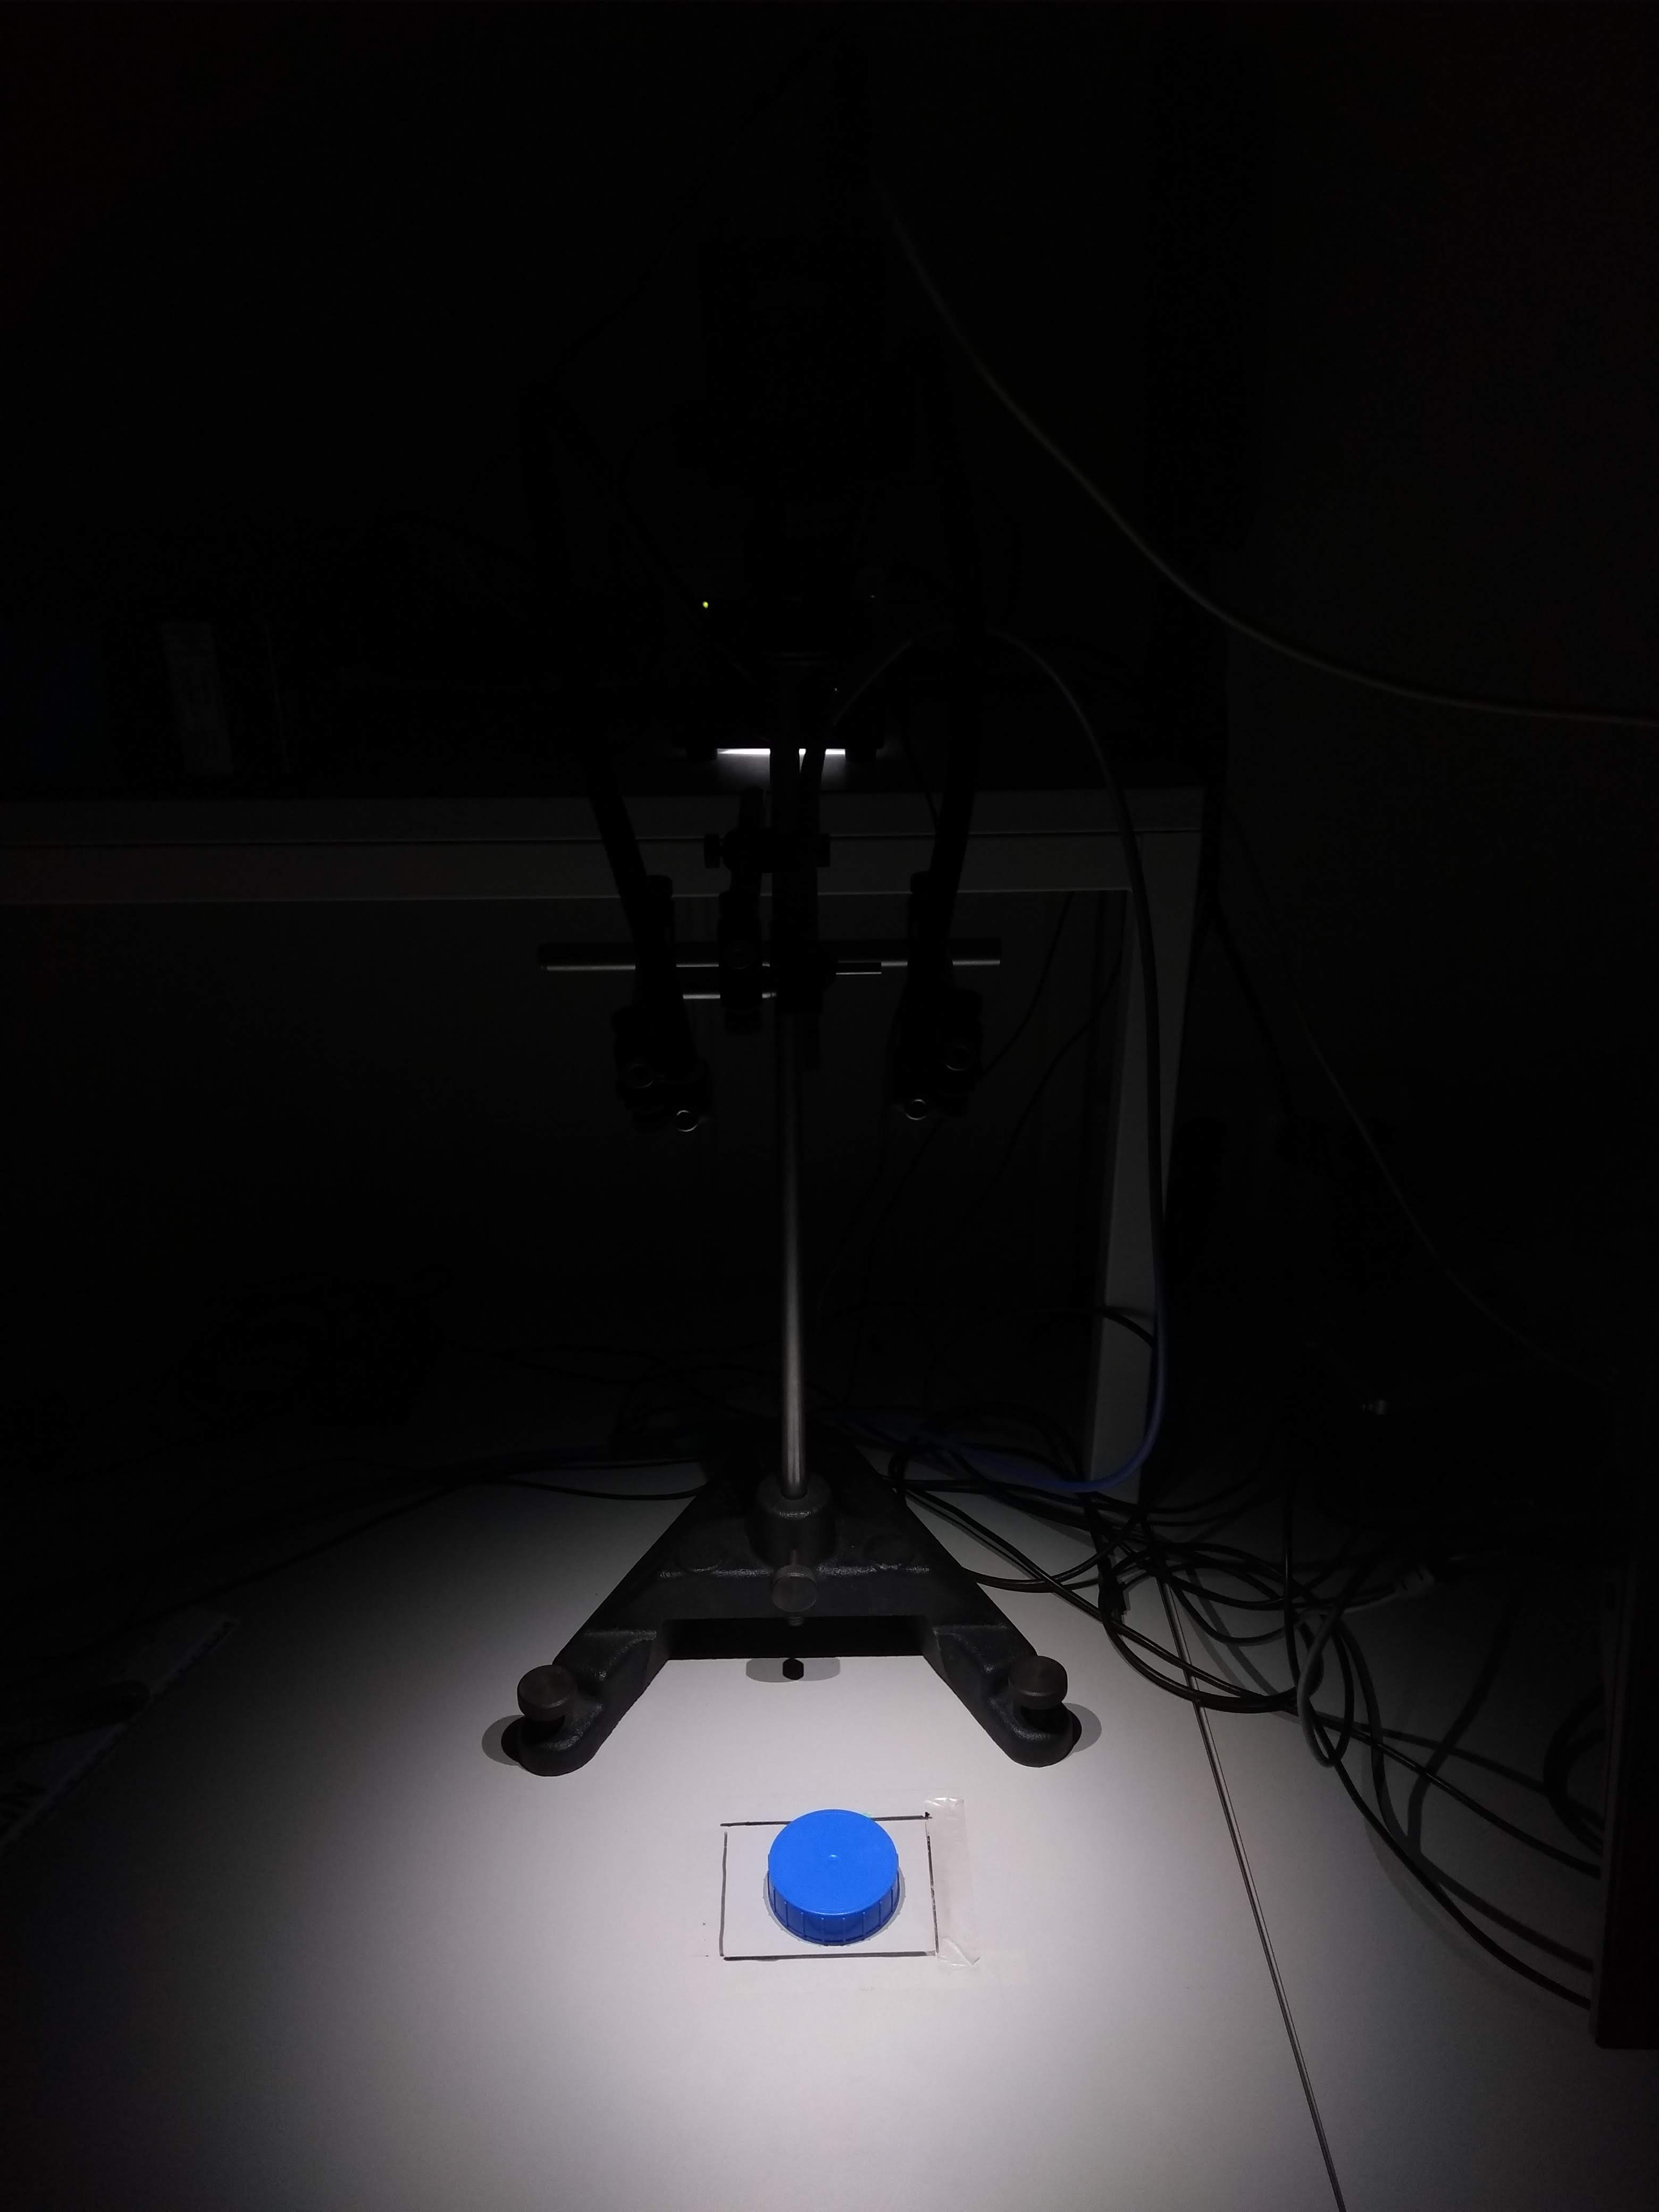
\includegraphics[width=1\textwidth]{figures/picture_taking_in_the_dark}
    \caption{Photo of the setup unlit}
    \label{fig:picture_of_setup_unlit}
\end{figure}


\subsection{Images}

\begin{figure}[h]
    \begin{subfigure}{0.5\textwidth}
        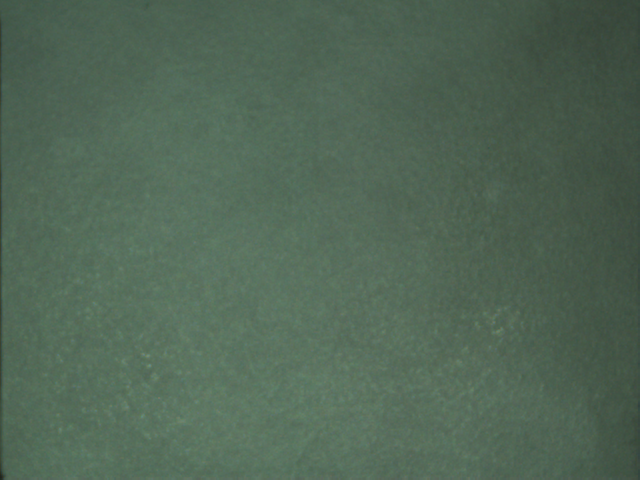
\includegraphics[width=0.9\linewidth, height=5cm]{figures/camera_pictures_png/001_background.png}
        \caption{001 Background, the reference picture}
        \label{fig:001_background}
        \end{subfigure}%
        \begin{subfigure}{0.5\textwidth}
        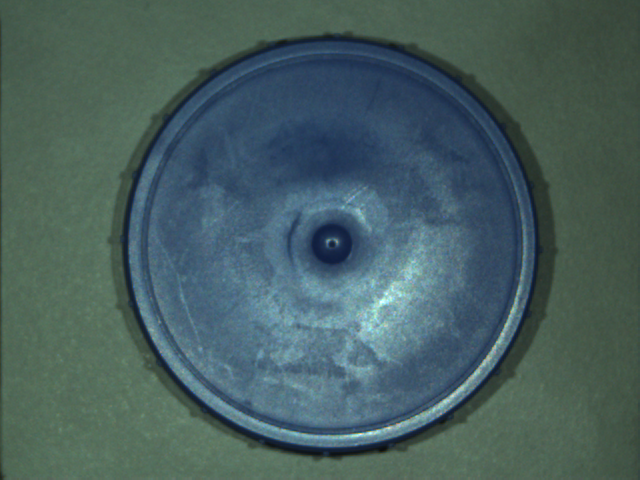
\includegraphics[width=0.9\linewidth, height=5cm]{figures/camera_pictures_png/002_blue_cap.png}
        \caption{002 Blue cap, the photo being analysed}
        \label{fig:002_blue_cap}
    \end{subfigure}
    
    \caption{The original images being used in figure \ref{fig:hadamard_division_blue_cap}}
    \label{fig:blue_cap_and_background}
\end{figure}



\begin{figure}[h]
    \begin{subfigure}{0.5\textwidth}
        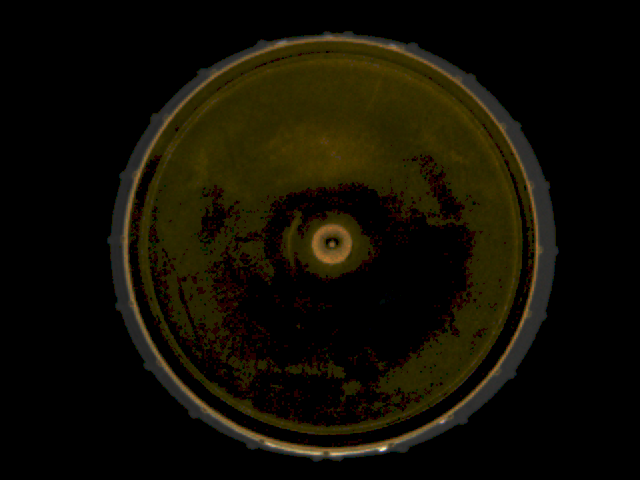
\includegraphics[width=0.9\linewidth, height=5cm]{figures/processed_camera_pictures/002_blue_cap_negative_difference.png} 
        \caption{Background image divided by blue cap image}
        \label{fig:002_blue_cap_negative_difference}
        \end{subfigure}%
        \begin{subfigure}{0.5\textwidth}
        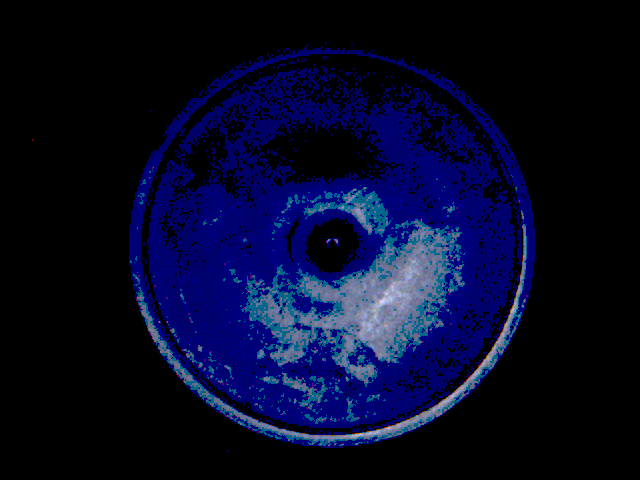
\includegraphics[width=0.9\linewidth, height=5cm]{figures/processed_camera_pictures/002_blue_cap_positive_difference.png}
        \caption{Blue cap image divided by background image}
        \label{fig:002_blue_cap_positive_difference}
    \end{subfigure}
    
    \caption{Hadamard division for the blue cap}
    \label{fig:hadamard_division_blue_cap}
\end{figure}


\subsection{Spectrum of camera}
Figure \ref{fig:relative_reflection_around_zero} shows nine plots, the first one shows the reference spectrum, the spectrum without any objects. The following eight plots shows the Relative Reflectance (\ref{eq:relative_reflectance}), their 

\begin{landscape}
\begin{figure}[t]
    \centering
    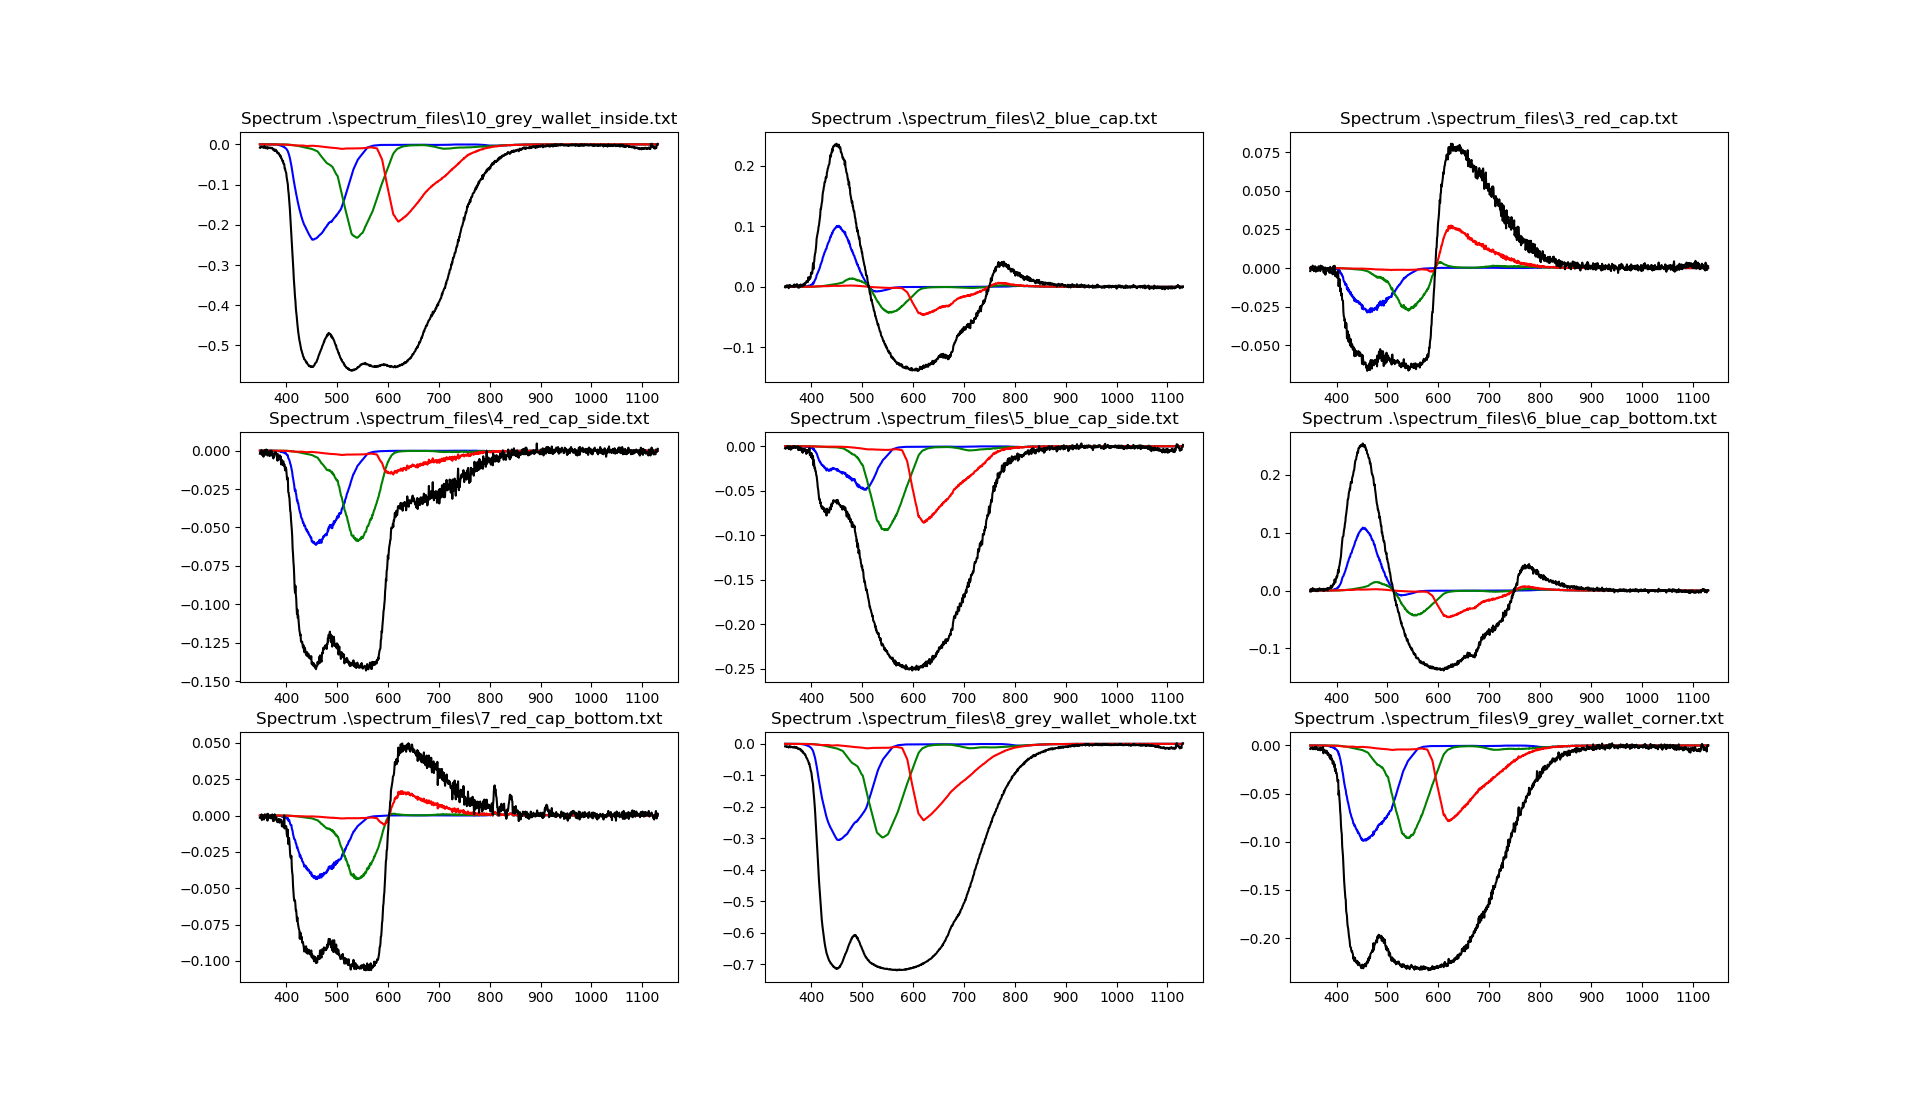
\includegraphics[width=1\paperwidth]{Plots/relative_reflectance_around_zero_with_qe_color_response.png}
    \caption{Relative reflection centered around zero}
    \label{fig:relative_reflection_around_zero}
\end{figure}
\end{landscape}


\subsection{Correlating Spectrometer to Camera}

After processing the images and spectrum as shown in figure \ref{fig:correlating_spectrum_and_image} 
